%\chapter{Limits of Random Variables}


\chapter{Limit Laws of Statistics}\label{S:LimitLawsStats}

\section{Convergence of Random Variables}\label{S:ConvOfRVs}

This important topic is concerned with the limiting behavior of sequences of RVs. 
We want to understand what it means for a sequence of random variables $\{X_n\}_{n=1}^{\infty} := X_1,X_2,\ldots$ to converge to another random variable $X$, when all RVs are defined on the same probability space $(\Omega,\mathcal{F},\p)$.
\[
\{X_i \}_{i=1}^n := X_1,X_2,X_3, \ldots X_{n-1}, X_n \qquad \text{as  $n \rightarrow \infty$ .}
\]
From a statistical or decision-making viewpoint, as you will see in Inference Theory I course, $n \rightarrow \infty$ is associated with the amount of data or information $\rightarrow \infty$.  
More abstractly, we are interested in what happens to the limiting RV $X := \lim_{n\to \infty} X_n$ when given the DFs $F_n(x)$ for each $X_n$. 

We need different notions of convergence to characterize such a behavior: two simplest behaviors are that the sequence eventually takes a constant value $\theta$, 
i.e. $X_n$ approaches $X \sim \pointmass(\theta)$ RV, or that values in the sequence continue to change but can be described by an unchanging probability distribution, i.e., $X_n$ approaches $X \sim F(x)$. See \url{https://en.wikipedia.org/wiki/Convergence_of_random_variables}.

Let us first refresh ourselves with notions of convergence, limits and continuity in the real line (\hyperref[S:AnalysisRefresher]{Sec.~\ref*{S:AnalysisRefresher}}) before proceeding further.

Can the sequences of $\{\pointmass(\theta_i=17)\}_{i=1}^{\infty}$ and $\{\pointmass(\theta_i=1/i)\}_{i=1}^{\infty}$ RVs be the same as the two sequences of real numbers $\{ x_i \}_{i=1}^{\infty} = 17, 17, 17, \ldots$ and $\{ x_i \}_{i=1}^{\infty} = \frac{1}{1},\frac{1}{2},\frac{1}{3}, \ldots$ we saw in Examples~\ref{EX:limOf17s} and \ref{EX:limin1overi}?


Yes why not -- just move to space of distributions over the reals! See Figure~\ref{F:SequenceOfPointMassRVS17And1Byi}.

\begin{figure}[htpb]
\caption{Sequence of $\{\pointmass(17)\}_{i=1}^{\infty}$ RVs (left panel) and $\{\pointmass(1/i)\}_{i=1}^{\infty}$ RVs (only the first seven are shown on right panel) and their limiting RVs in red.\label{F:SequenceOfPointMassRVS17And1Byi}}
\centering   \makebox{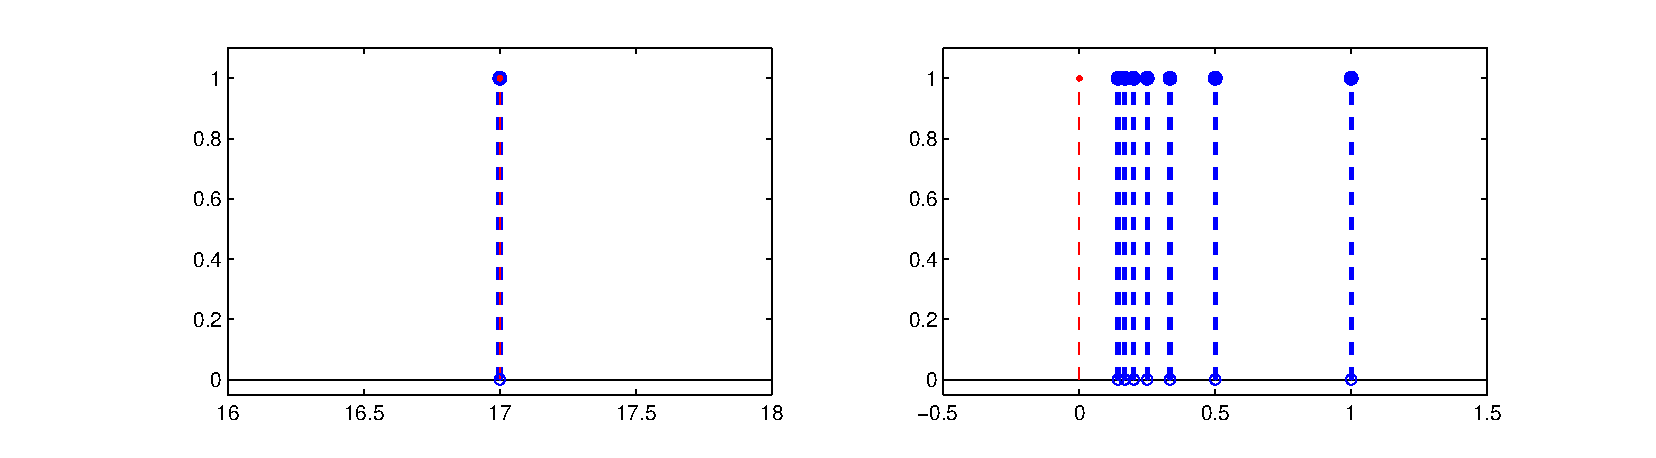
\includegraphics[width=6.5in]{figures/SequenceOfPointMassRVS17And1Byi}}
\end{figure}

\begin{classwork}[Convergence of $X_i \sim \normal(0,1/i)$]\label{CW:Normal01bynConvToPointMass0}
Suppose you are given an independent sequence of RVs $\{X_i \}_{i=1}^n$, where $X_i \sim \normal(0,1/i)$.  How would you talk about the convergence of $X_n \sim \normal(0,1/n)$ as $n$ approaches $\infty$ ?  Take a look at \hyperref[F:PlotNormal01bynConvToPointMass0]{Figure \ref*{F:PlotNormal01bynConvToPointMass0}} for insight.  The probability mass of $X_n$ increasingly concentrates about $0$ as $n$ approaches $\infty$ and the variance $1/n$ approaches $0$, as depicted in \hyperref[F:PlotNormal01bynConvToPointMass0]{Figure \ref*{F:PlotNormal01bynConvToPointMass0}}.  Based on this observation, can we expect $\lim_{n \rightarrow \infty} X_n = X$, where the limiting RV $X \sim \pointmass(0)$ ?

The answer is {\bf no}.  This is because $\p(X_n=X)=0$ for any $n$, since $X \sim \pointmass(0)$ is a discrete RV with exactly one outcome $0$ and $X_n \sim \normal(0,1/n)$ is a continuous RV for every $n$, however large.  In other words, a continuous RV, such as $X_n$, has $0$ probability of realizing any single real number in its support, such as $0$.    
\begin{figure}[htpb]
\caption{Distribution functions of several $\normal(\mu,\sigma^2)$ RVs for $\sigma^2 = 1,\frac{1}{10},\frac{1}{100},\frac{1}{1000}$.\label{F:PlotNormal01bynConvToPointMass0}}
\centering   \makebox{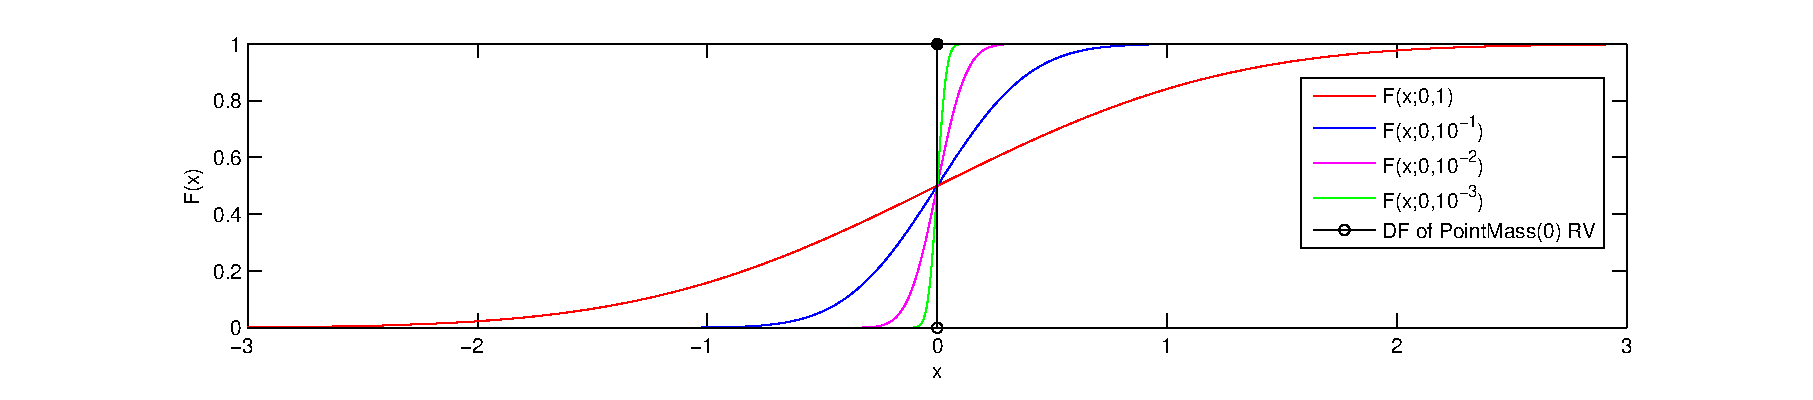
\includegraphics[width=6.5in]{figures/PlotNormal01bynConvToPointMass0}}
\end{figure}
\end{classwork}

Thus, we need more sophisticated notions of convergence for sequences of RVs.  Two such notions are formalized next as they are minimal prerequisites for a clear understanding of two basic propositions in Statistics :
\begin{enumerate} 
\item Law of Large Numbers,
\item Central Limit Theorem,
%\item Gilvenko-Cantelli Theorem.
\end{enumerate}

\begin{definition}[Convergence in Distribution (or Weakly, or in Law)]\label{D:ConvInDist}
Let $X_1,X_2,\ldots,$ be a sequence of RVs and let $X$ be another RV.  Let $F_n$ denote the DF of $X_n$ and $F$ denote the DF of $X$.  The we say that $X_n$ converges to $X$ in distribution, and write:
\[
X_n \rightsquigarrow X
\]
if for any real number $t$ at which $F$ is continuous,
\[
\lim_{n \rightarrow \infty} F_n(t) = F(t) \qquad \text{[in the sense of \hyperref[D:LimitofRealFunction]{Definition \ref*{D:LimitofRealFunction}}].}
\]
The above limit, by \eqref{E:DF} in our \hyperref[D:DF]{Definition \ref*{D:DF}} of a DF, can be equivalently expressed as follows: 
\begin{eqnarray}
& & \lim_{n \rightarrow \infty} \p( \ \{\omega: X_n(\omega) \leq  t \} \ )= 
\p( \ \{\omega: X(\omega) \leq  t \} \ ), \notag \\
&\text{i.e.~} & \p( \ \{\omega: X_n(\omega) \leq t \} \ ) \rightarrow \p( \ \{\omega: X(\omega) \leq  t \} \ ), \quad \text{as} \quad n \rightarrow \infty \notag \ .
\end{eqnarray}
\end{definition}

Let us revisit the problem of convergence in \hyperref[CW:Normal01bynConvToPointMass0]{Classwork \ref*{CW:Normal01bynConvToPointMass0}} armed with our new notions of convergence.
\begin{example}[Convergence in distribution]\label{EX:Normal01bynConvinDistToPointMass0}
Suppose you are given an independent sequence of RVs $\{X_i \}_{i=1}^n$, where $X_i \sim \normal(0,1/i)$ with DF $F_n$ and let $X \sim \pointmass(0)$ with DF $F$.  We can formalize our observation in \hyperref[CW:Normal01bynConvToPointMass0]{Classwork \ref*{CW:Normal01bynConvToPointMass0}} that $X_n$ is concentrating about $0$ as $n \to \infty$ by the statement:
\[
\text{$X_n$ is converging in distribution to $X$, ie,} \qquad X_n \rightsquigarrow X \ .
\]
{\normalsize
\begin{proof}
To check that the above statement is true we need to verify that the definition of convergence in distribution is satisfied for our sequence of RVs $X_1,X_2,\ldots$ and the limiting RV $X$.  Thus, we need to verify that for any continuity point $t$ of the $\pointmass(0)$ DF $F$, $\lim_{n \to \infty} F_n(t)=F(t)$.  First note that 
\[
X_n \sim \normal(0,1/n) \implies Z := \sqrt{n} X_n \sim \normal(0,1) \ ,
\]
and thus
\[
F_n(t) = \p(X_n < t) = \p(\sqrt{n} X_n < \sqrt{n} t) = \p(Z < \sqrt{n} t) \ .
\]
The only discontinuous point of $F$ is $0$ where $F$ jump from $0$ to $1$.  

When $t < 0$, $F(t)$, being the constant $0$ function over the interval $(-\infty,0)$, is continuous at $t$.  Since $\sqrt{n} t \to -\infty$, as $n \to \infty$,
\[
\lim_{n \to \infty} F_n(t)  = \lim_{n \to \infty} \p(Z < \sqrt{n} t) = 0 = F(t) \ .
\]
And, when $t >0$, $F(t)$, being the constant $1$ function over the interval $(0,\infty)$, is again continuous at $t$.  Since $\sqrt{n} t \to \infty$, as $n \to \infty$,
\[
\lim_{n \to \infty} F_n(t)  = \lim_{n \to \infty} \p(Z < \sqrt{n} t) = 1 = F(t) \ .
\]
Thus, we have proved that $X_n \rightsquigarrow X$ by verifying that for any $t$ at which the $\pointmass(0)$ DF $F$ is continuous, we also have the desired equality: $\lim_{n \to \infty} F_n(t)=F(t)$.
\end{proof}
However, note that 
\[
F_n(0)=\frac{1}{2} \neq F(0)=1 \ ,
\]
and so convergence fails at $0$, i.e.~$\lim_{n \to \infty}F_n(t) \neq F(t)$ at $t=0$.  But, $t=0$ is not a continuity point of $F$ and the definition of convergence in distribution only requires the convergence to hold at continuity points of $F$.
}
\end{example}

\begin{figure}[htbp]
\begin{center}
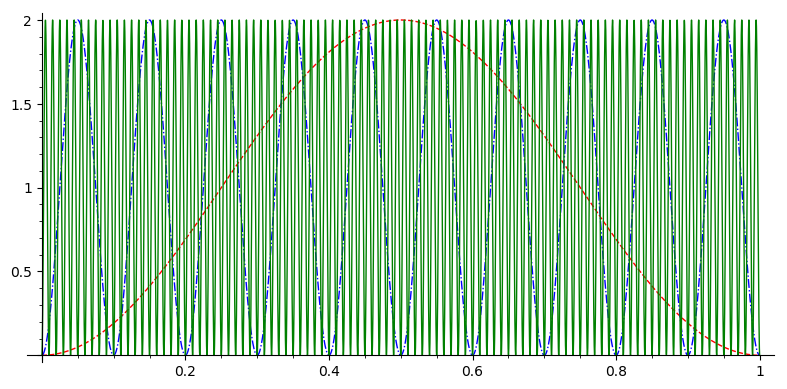
\includegraphics[width=10cm]{figures/PDFOf1minusCos2PinxOn01OscillatesIndefinitely.png}
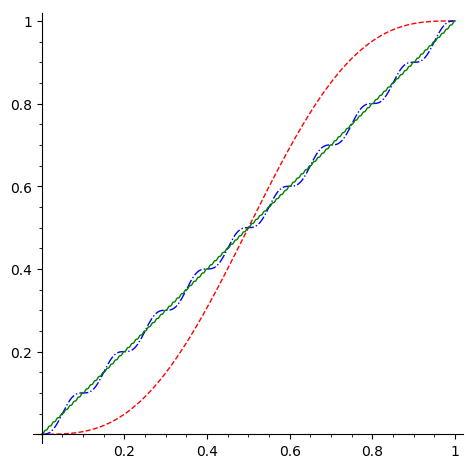
\includegraphics[width=5cm]{figures/DFOf1minusCos2PinxOn01To1ApproachesDFOfUniform01.png}
\caption{PDF $f_{X_n}(x) := \BB{1}_{(0,1)}(x)(1-\cos(2\pi n x))$ of the RV $X_n$ [the left sub-figure] and its DF $F_n(x) := \int_{-\infty}^x\BB{1}_{(0,1)}(v)(1-\cos(2\pi n v))dv$ [the right sub-figure], for $n =1$ [red '- -'], $n=10$ [blue '-.'], and $n=100$ [green '-'], respectively. One can see clear convergence of the DFs $F_n$ to $\BB{1}_{(0,1)}(x)x$, the DF of the $\uniform(0,1)$ RV, while the corresponding PDFs $f_n(x)$ keep oscillating wildly with $n$ across $[0,2]$ about $\BB{1}_{(0,1)}(x)$, the PDF of the $\uniform(0,1)$ RV $X$. Thus giving a counter-example to the claim that convergence in DFs does not imply convergence in PDFs.\label{F:ScheffesThmCounterExample}}
\end{center}
\end{figure}
Convergence in distribution does not in general imply that the sequence of corresponsing probability density functions will also converge. 
Consider for example RV $X_n$ with density $\BB{1}_{(0,1)}(x)(1-\cos(2\pi n x))$. 
These RVs converge in distribution to $X \sim \uniform(0,1)$, but their densities (PDFs) do not converge at all as evident in Figure~\ref{F:ScheffesThmCounterExample}. 

\begin{prop}[Scheff\'e's Theorem]
According to {\bf Scheff\'e's Theorem} convergence of the probability density function (for a continuous RV) or probability mass function (for a discrete RV) implies convergence in distribution.
\begin{proof}
We will state this without a Proof here as Proof of the Theorem requires measure theory in generality \footnote{See \url{https://en.wikipedia.org/wiki/Scheff\%C3\%A9\%27s_lemma}.}. However, you should be able to see why convergence of PMFs $f_n(x)$ for discrete RVs $X_n$, to $f(x)$, the PMF of another discrete RV $X$, implies convergence in their corresponding DFs, i.e., $F_n(x) \to F(x)$ for each $x$ as $n \to \infty$. 
\end{proof}
\end{prop}

Since $F(x) = \p(X \leq x)$, convergence in distribution means that the probability for $X_n$ to be in a given range is approximately equal to the probability that the value of the limiting RV $X$ is in that range, provided $n$ is sufficiently large. 

Thus, for a discrete sequence of RVs $X_n$`n to converge in distribution to another discrete RV $X$ taking values in $\mathbb{Z}_+ = \{0,1,2,\ldots\}$, it is sufficient to show that $\lim_{n \to \infty}\p(X_n = x) = \p(X=x)$ for each $x \in \mathbb{Z_+}$.  
We will use this fact to prove why we can approximate $\binomial$ RVs by a $\poisson$ under some limiting conditions.

\begin{example}[$\binomial(n,\lambda/n) {\rightsquigarrow} \poisson(\lambda)$]\label{EgBinomialConvergesInDistToPoisson}
In several situations, as we saw already, it becomes cumbersome to model the events using the $\binomial(n,\theta)$ RV, especially when when the parameter $\theta \propto 1/n$ and the events become rare.  

\begin{center}
\begin{frame}
{$\binomial(n,\lambda/n)$ converges in distribution to $\poisson(\lambda)$ as $n \to \infty$, $\theta=\lambda/n \to 0$}
\end{frame}
\end{center}

However, for some real parameter $\lambda>0$, the $\binomial(n,\lambda/n)$ RV with probability of the number of successes in $n$ trials, with per-trial success probability $\lambda/n$, approaches the Poisson distribution with expectation $\lambda$, as $n$ approaches $\infty$ (actually, it converges in distribution).  
The $\poisson(\lambda)$ RV is much simpler to work with than the combinatorially laden $\binomial(n,\theta=\lambda/n)$ RV.  We sketch the details of this next.

Let $X_n \sim \binomial(n,\theta=\lambda/n)$ and $Y \sim \poisson(\lambda)$ and let $\lambda=n\theta$ remain constant as  $n \to \infty$, $\theta \to 0$.  
We need to show that $\lim_{n \to \infty} \p(X_n=x) = \p(Y=x) = e^{-\lambda}\lambda^x/x!$ for any $x \in \{0,1,2,3,\ldots,n\}$. 
%{\normalsize
\begin{eqnarray}
\p(X=x)
&=&
\binom{n}{x} \left( \frac{\lambda}{n} \right)^x \left( 1- \frac{\lambda}{n} \right)^{n-x} \notag \\
&=& \frac{n(n-1)(n-2)\cdots(n-x+1)}{x(x-1)(x-2)\cdots (2)(1)}
\left( \frac{\lambda^x}{n^x} \right)
\left( 1- \frac{\lambda}{n} \right)^n
\left( 1- \frac{\lambda}{n} \right)^{-x} \notag \\
&=&
\overbrace{\left( \frac{n}{n} \right) \left( \frac{n-1}{n} \right) \left( \frac{n-2}{n} \right) \cdots \left( \frac{n-x+1}{n} \right)}
\overbrace{\left( \frac{\lambda^x}{x!} \right)}
\underbrace{\left( 1- \frac{\lambda}{n} \right)^n}
\underbrace{\left( 1- \frac{\lambda}{n} \right)^{-x}}  \notag \\
\end{eqnarray}

As $n \to \infty$, the expression below the first overbrace $\to 1$, while that below the second overbrace, being independent of $n$ remains the same.  By the elementary examples of limits
%\remove{
\ref*{EX:LimitExpofLambda} and \ref*{EX:Limit1MinusLambdaOverNToMinusK}%}
, as $n \to \infty$, the expression over the first underbrace approaches $e^{-\lambda}$ while that over the second underbrace approaches $1$.  Finally, we get the desired limit:

\[
\lim_{n \to \infty} \p(X=x)
= \frac{ e^{-\lambda} \lambda^x}{x!}  \ .
\]
%}
\end{example}

The second notion of convergence of RVs is convergence in probability.

\begin{definition}[Convergence in Probability]\label{D:ConvInProb}
Let $X_1,X_2,\ldots,$ be a sequence of RVs and let $X$ be another RV.  Let $F_n$ denote the DF of $X_n$ and $F$ denote the DF of $X$.  The we say that $X_n$ converges to $X$ in probability, and write:
\[
X_n \overset{\p}{\longrightarrow} X
\]
if for every real number $\epsilon > 0$,
\[
\lim_{n \rightarrow \infty} \p(|X_n-X|> \epsilon) = 0 \qquad \text{[in the sense of \hyperref[D:LimitofRealFunction]{Definition \ref*{D:LimitofRealFunction}}].}
\]
Once again, the above limit, by \eqref{E:ProbOfRV} in our \hyperref[D:RV]{Definition \ref*{D:RV}} of a RV, can be equivalently expressed as follows: 
\[
\lim_{n \rightarrow \infty} \p( \ \{\omega: |X_n(\omega) - X(\omega)| > \epsilon\} \ )=0, \qquad \text{ie,} \qquad \p( \ \{\omega: |X_n(\omega) - X(\omega)| > \epsilon\} \ ) \rightarrow 0, \quad \text{as} \quad n \rightarrow \infty \ .
\]
\end{definition}
 
For the same sequence of RVs in  \hyperref[CW:Normal01bynConvToPointMass0]{Classwork \ref*{CW:Normal01bynConvToPointMass0}} and \hyperref[EX:Normal01bynConvinDistToPointMass0]{Example \ref*{EX:Normal01bynConvinDistToPointMass0}} we are tempted to ask whether $X_n \sim \normal(0,1/n)$ converges in probability to $X \sim \pointmass(0)$, i.e.~whether $X_n \overset{\p}{\longrightarrow} X$.  We need some elementary inequalities in Probability to help us answer this question.  We visit these inequalities next.


\begin{prop}[Markov's Inequality]
Let $(\Omega,\C{F},P)$ be a probability triple and let $X=X(\omega)$ be a non-negative RV.  Then,
\begin{equation}\label{E:MarkovNeq}
\p(X \geq \epsilon) \leq \frac{\e(X)}{\epsilon}, \qquad \text{for any} \quad \epsilon > 0 \ .
\end{equation}
{\normalsize
\begin{proof}
\begin{eqnarray}
X &=& X \BB{1}_{ \{y: y \geq \epsilon \} } (x) + X \BB{1}_{ \{y: y < \epsilon \} } (x) \notag \\
&\geq& X \BB{1}_{ \{y: y \geq \epsilon \} } (x) \notag \\
&\geq& \epsilon  \BB{1}_{ \{y: y \geq \epsilon \} } (x) \notag \\
\end{eqnarray}
Finally, taking expectations on both sides of the above inequality and then using the fact that the expectation of an indicator function of an event is simply the probability of that event \eqref{E:ExpectationofIndicator}, we get the desired result:
\[
\e(X) \geq \epsilon \e( \BB{1}_{ \{y: y \geq \epsilon \} } (x)) = \epsilon \p(X \geq \epsilon) \ .
\]
\end{proof}
}
\end{prop}
Let us look at some immediate consequences of Markov's inequality.
\begin{prop}[Chebychev's Inequality]
For {\bf any} RV $X$ and any $\epsilon > 0$,
\begin{eqnarray}
\p(|X| > \epsilon) &\leq& \frac{\e(|X|)}{\epsilon} \label{E:ChebychevNeq1} \\
\p(|X| > \epsilon) = \p(X^2 \geq \epsilon^2) &\leq& \frac{\e(X^2)}{\epsilon^2} \label{E:ChebychevNeq2} \\
\p(|X-\e(X)| \geq \epsilon) = \p((X-\e(X))^2 \geq \epsilon^2) &\leq& \frac{\e(X-\e(X))^2}{\epsilon^2}  = \frac{\V(X)}{\epsilon^2}  \label{E:ChebychevNeq3} 
\end{eqnarray}
{\normalsize
\begin{proof}
All three forms of Chebychev's inequality are mere corollaries (careful reapplications) of Markov's inequality.
\end{proof}
}
\end{prop}

Armed with Markov's inequality we next enquire the convergence in probability for the sequence of RVs in \hyperref[CW:Normal01bynConvToPointMass0]{Classwork \ref*{CW:Normal01bynConvToPointMass0}} and \hyperref[EX:Normal01bynConvinDistToPointMass0]{Example \ref*{EX:Normal01bynConvinDistToPointMass0}}.

\begin{example}[Convergence in probability]\label{EX:Normal01bynConvinProbToPointMass0}
Does the the sequence of RVs $\{X_n\}_{n=1}^{\infty}$, where $X_n \sim \normal(0,1/n)$, converge in probability to $X \sim \pointmass(0)$, i.e.~does $X_n \overset{\p}{\longrightarrow} X$ ?

To find out if $X_n \overset{\p}{\longrightarrow} X$, we need to show that for any $\epsilon >0$, $\lim_{n \to \infty} \p(|X_n-X|>\epsilon)=0$.

Let $\epsilon$ be any real number greater than $0$, then
\begin{eqnarray}
\p(|X_n|>\epsilon) &=& \p(|X_n|^2 > \epsilon^2) \notag \\
&\leq& \frac{\e(X_n^2)}{\epsilon^2} \qquad \text{[by Markov's Inequality \eqref{E:MarkovNeq}]} \notag \\
&=& \frac{\frac{1}{n}}{\epsilon^2} \to 0, \quad \text{as} \quad n \to \infty \qquad \text{[in the sense of \hyperref[D:LimitofRealFunction]{Definition \ref*{D:LimitofRealFunction}}].} \notag
\end{eqnarray}
Hence, we have shown that for any $\epsilon >0$, $\lim_{n \to \infty} \p(|X_n-X|>\epsilon)=0$ and therefore by \hyperref[D:ConvInProb]{Definition \ref*{D:ConvInProb}}, $X_n \overset{\p}{\longrightarrow} X$ or $X_n \overset{\p}{\longrightarrow} 0$.  

{\normalsize
{\bf Convention:} When $X$ has a $\pointmass(\theta)$ distribution and $X_n \overset{\p}{\longrightarrow} X$, we simply write $X_n \overset{\p}{\longrightarrow} \theta$.
}
\end{example}

\begin{definition}[Convergence Almost Surely (or with Probability $1$)]
To say that the sequence of RVs $\{X_n\}_{n=1}^{\infty}$ converges almost surely (or with probability $1$ or strongly) towards another RV $X$ on the same probability space $(\Omega,\mathcal{F},\p)$, as denoted by
\[
X_n \overset{a.s.}{\to} X
\]
means that
\[
\p \left( \{ \lim_{n \to \infty} X_n = X \} \right) = 1 \quad \iff \quad \p \left( \{\omega \in \Omega : \lim_{n \to \infty} X_n(\omega) = X(\omega)\} \right) = 1.
\]
This means that the values of $X_n$ approach the value of $X$, in the sense that events for which $X_n$ does not converge to $X$ have probability $0$.
\end{definition}

Other notions of convergence are termed sure convergence or pointwise convergence, such as convergence in mean. 
But the above three types of convergence are elementary. % and enough to appreciate the subtle issues with convergence of random variables.

\subsection{Properties of Convergence of RVs$^{**}$}

We will merely state some properties (without proofs that are hyper-linked for the curious student as they are advanced for this course) and relations between the three notions of convergence with some examples to better appreciate the subtleties among them. 
You will study the proofs of these statements in Probability Theory II. 
Just remember that subtle implication relations exist between the three notions.


%Now that we have been introduced to three notions of convergence for sequences of RVs we can begin to appreciate the  construction of limiting random variables from existing ones. % We will see a limiting sum of $n$ independent $\bernoulli(\theta)$ RVs as $n \to \infty$ and $\theta \to 0$ such that $n \theta = \lambda$. %  statements of the basic limit theorems of Statistics.  
%But first we need some analytic tools.

%But first we formally define a statistic.


\bit
\item Convergence almost surely implies convergence in probability\footnote{{\tiny \url{https://en.wikipedia.org/wiki/Proofs\_of\_convergence\_of\_random\_variables\#Convergence\_almost\_surely\_implies\_convergence\_in\_probability}}}
\[
\boxed{X_n \overset{a.s.}{\to} X \implies X_n \overset{\p}{\to} X \enspace .}
\]
\item By the Borel-Cantelli Lemma \footnote{{\tiny \url{https://en.wikipedia.org/wiki/Borel\%E2\%80\%93Cantelli\_lemma}}}, convergence in probability does not imply almost sure convergence in the discrete case \footnote{{\tiny \url{https://en.wikipedia.org/wiki/Proofs_of_convergence_of_random_variables\#Convergence_in_probability_does_not_imply_almost_sure_convergence_in_the_discrete_case}}}
\item Convergence in probability implies convergence in distribution \footnote{{\tiny \url{https://en.wikipedia.org/wiki/Proofs_of_convergence_of_random_variables\#Convergence_in_probability_implies_convergence_in_distribution}}} 
\[
\boxed{X_n \overset{\p}{\to} X \implies X_n \rightsquigarrow X \enspace .}
\]
\item Convergence in distribution to a constant $\theta$ implies convergence in probability to $\theta$: \footnote{{\tiny \url{https://en.wikipedia.org/wiki/Proofs_of_convergence_of_random_variables\#Convergence_in_distribution_to_a_constant_implies_convergence_in_probability}}}
\[
X_n \rightsquigarrow \pointmass(\theta) \implies X_n \overset{\p}{\to} \pointmass(\theta) \enspace . 
\] 
\item In general, convergence in distribution does not imply convergence in probability.  %\footnote{{\tiny \url{}}} 
\eit


\section{Law of Large Numbers}

\begin{prop}[Law of Large Numbers (LLN): $\overline{X}_n \overset{\p}{\longrightarrow} \e(X_1)$]
If we are given a sequence if independent and identically distributed RVs, $X_1,X_2,\ldots \overset{\IID}{\sim} X_1$ and if $\e(X_1)$ exists, as per \eqref{E:ExpectationExists}, i.e., $\e(\abs(X_1))< \infty$, and the variance is finite, i.e., $\V(X_1) < \infty$, then the sample mean $\overline{X}_n$ converges in probability to the expectation of any one of the IID RVs, say $\e(X_1)$ by convention.  More formally, we write:
\[
\text{If} \quad X_1,X_2,\ldots \overset{\IID}{\sim} X_1 \ \text{and if } \ \e(X_1) \ \text{exists, then } \ \overline{X}_n \overset{\p}{\longrightarrow} \e(X_1) \ .
\]
{\normalsize
\begin{proof}
Because $\V(X_1) < \infty$, we have:
\begin{eqnarray}
\p(| \overline{X}_n - \e(\overline{X}_n) | \geq \epsilon)
&=& \frac{\V(\overline{X}_n)}{\epsilon^2} \qquad \text{{\scriptsize [by applying Chebychev's inequality \eqref{E:ChebychevNeq3} to the RV $\overline{X}_n$]}} \notag \\
&=& \frac{\frac{1}{n}\V(X_1)}{\epsilon^2} \qquad \text{{\scriptsize [by the IID assumption of $X_1,X_2,\ldots$ we can apply \eqref{E:VarOfSampleMeanOfIIDSeq}]}} \notag 
\end{eqnarray}
Therefore, for any given $\epsilon>0$,
\begin{eqnarray}
\p(| \overline{X}_n - \e(X_1) | \geq \epsilon)
&=&  \p(| \overline{X}_n - \e(\overline{X}_n) | \geq \epsilon) \qquad \text{{\scriptsize [by the IID assumption of $X_1,X_2,\ldots$,  $\e(\overline{X}_n)=\e(X_1)$, as per \eqref{E:ExpOfSampleMeanOfIDSeq}]}} \notag \\
&=&  \frac{\frac{1}{n}\V(X_1)}{\epsilon^2} \to 0, \quad \text{as} \quad n \to \infty \ , \notag
\end{eqnarray}
or equivalently, $\lim_{n \to \infty} \p(| \overline{X}_n - \e(X_1) | \geq \epsilon) = 0$.  And the last statement is the definition of the claim made by the law of large numbers (LLN), namely that $\overline{X}_n \overset{\p}{\longrightarrow} \e(X_1)$ .
\end{proof}
}

\begin{prop}[Weak Law of Large Numbers (WLLN): $\overline{X}_n \rightsquigarrow \pointmass(\e(X_1))$]
If we are given a sequence of independently and identically distributed (IID) RVs, $X_1,X_2,\ldots \overset{\IID}{\sim} X_1$ and if $\e(X_1)$ exists, i.e.~$\e(\abs(X)) < \infty$, then the sample mean $\overline{X}_n$ converges in distribution to the expectation of any one of the IID RVs, say $\pointmass(\e(X_1))$ by convention.  More formally, we write:
\[
\text{If} \quad X_1,X_2,\ldots \overset{\IID}{\sim} X_1 \ \text{and if } \ \e(X_1) \ \text{exists, then } \ \overline{X}_n \rightsquigarrow \pointmass(\e(X_1)) \ \text{ as } n\to\infty \enspace .
\]
\end{prop}

{\normalsize
\begin{proof}
Our proof now is based on the convergence of characteristic functions (CFs) pointwise to the CF of the limiting RV, as this implies, by L\'evy's Continuity Theorem on CFs \footnote{\url{https://en.wikipedia.org/wiki/L\%C3\%A9vy\%27s_continuity_theorem}}, the convergence of the corresponding distribution functions (DFs).  

First, the CF of $\pointmass(\e(X_1))$ is 
\[
\e(e^{\imath t \e(X_1)})=e^{\imath t \e(X_1)} \enspace,
\]
since $\e(X_1)$ is just a constant, i.e., a $\pointmass$ RV that puts all of its probability mass at $\e(X_1)$.  

Second, the CF of $\ol{X}_n$ is 
\begin{align*}
\e \left( e^{\imath t \ol{X}_n}\right)
&= \e \left( e^{\imath t \frac{1}{n} \sum_{k=1}^n X_k} \right) = \e \left( \prod_{k=1}^n e^{\imath t X_k/n} \right) = \prod_{k=1}^n \e \left( e^{\imath t X_k/n} \right) = \prod_{k=1}^n \cf_{X_k}(t/n)\\ 
&= \prod_{k=1}^n \cf_{X_1}(t/n) =\left(\cf_{X_1}(t/n)\right)^n \enspace .
\end{align*}

Let us recall Landau's ``small o'' notation for the relation between two functions.  
We say,  $f(x)$ is {\bf small o} of $g(x)$ if $f$ is dominated by $g$ as $x \to \infty$, i.e., $\frac{|f(x)|}{|g(x)|} \to 0$ as $x \to \infty$.  
More formally, for every $\epsilon > 0$, there exists an $x_{\epsilon}$ such that for all $x > x_{\epsilon}$ $|f(x)| < \epsilon |g(x)|$.  
For example, $\log(x)$ is $o(x)$, $x^2$ is $o(x^3)$ and $x^m$ is $o(x^{m+1})$ for $m\geq 1$.  

Third, we can expand any CF whose expectation exists as a Taylor series with a remainder term that is $o(t)$ as follows:
\[
\cf_X(t) = 1 + \imath t \e(X) + o(t) \enspace .
\]
Hence,
\[
\cf_{X_1}(t/n) = 1 + \imath \frac{t}{n} \e(X_1) + o\left(\frac{t}{n}\right) 
\]
and
\[
E \left( e^{\imath t \ol{X}_n}\right) = \left( 1 + \imath \frac{t}{n} \e(X_1) + o\left(\frac{t}{n}\right) \right)^n
\to e^{\imath t \e(X_1)} \text{ as } n \to \infty \enspace .
\]
For the last limit we have used $\left( 1+\frac{x}{n}\right)^n \to e^x$ as $n \to \infty$.

Finally, we have shown that $E \left( e^{\imath t \ol{X}_n}\right)$, the CF of the $n$-sample mean RV $\ol{X}_n$, converges to $\e(e^{\imath t \e(X_1)})=e^{\imath t \e(X_1)}$, the CF of the $\pointmass(\e(X_1))$ RV, as the sample size $n$ tends to infinity.
\end{proof}
%%%%%%%%%%%%%%%%%%%%%%%%%%%%%%%%%%%--too heavy for Inference Course - not introduced to conv in prob, Markov ineq or Chebychev ineq
%\begin{proof}
%For simplicity, we will prove a slightly weaker result by assuming finite variance of $X_1$.  Suppose $\V(X_1) < \infty$, then:
%\begin{eqnarray}
%\p(| \overline{X}_n - \e(\overline{X}_n) | \geq \epsilon)
%&=& \frac{\V(\overline{X}_n)}{\epsilon^2} \qquad \text{{\scriptsize [by applying Chebychev's inequality \eqref{E:ChebychevNeq3} to the RV $\overline{X}_n$]}} \notag \\
%&=& \frac{\frac{1}{n}\V(X_1)}{\epsilon^2} \qquad \text{{\scriptsize [by the IID assumption of $X_1,X_2,\ldots$ we can apply \eqref{E:VarOfSampleMeanOfIIDSeq}]}} \notag 
%\end{eqnarray}
%Therefore, for any given $\epsilon>0$,
%\begin{eqnarray}
%\p(| \overline{X}_n - \e(X_1) | \geq \epsilon)
%&=&  \p(| \overline{X}_n - \e(\overline{X}_n) | \geq \epsilon) \qquad \text{{\scriptsize [by the IID assumption of $X_1,X_2,\ldots$,  $\e(\overline{X}_n)=\e(X_1)$, as per \eqref{E:ExpOfSampleMeanOfIDSeq}]}} \notag \\
%&=&  \frac{\frac{1}{n}\V(X_1)}{\epsilon^2} \to 0, \quad \text{as} \quad n \to \infty \ , \notag
%\end{eqnarray}
%or equivalently, $\lim_{n \to \infty} \p(| \overline{X}_n - \e(X_1) | \geq \epsilon) = 0$.  And the last statement is the Definition of the claim made by the weak law of large numbers (LLN), namely that $\overline{X}_n \overset{\p}{\longrightarrow} \e(X_1)$ .
%\end{proof}
%%%%%%%%%%%%%%%%%%%%%%%%%%%%%%%%%%%
}
\end{prop}


\subsubsection{Heuristic Interpretation of LLN}  
The distribution of the sample mean RV $\overline{X}_n$ obtained from an independent and identically distributed sequence of RVs $X_1,X_2,\ldots$ {\scriptsize [i.e.~all the RVs $X_i$'s are independent of one another and have the same distribution function, and thereby the same expectation, variance and higher moments]}, concentrates around the expectation of any one of the RVs in the sequence, say that of the first one $\e(X_1)$ {\scriptsize [without loss of generality]}, as $n$ approaches infinity.  See Figure~\ref{F:RunningMeansFairDieFairCoinUnif01Exp1By10} for examples of 20 replicates of the sample mean of IID sequences from four RVs.  All the sample mean trajectories converge to the corresponding population mean. 

\begin{figure}[htpb]
\caption{Sample mean $\ol{X}_n$ as a function of sample size $n$ for 20 replications from independent realizations of a fair die (blue), fair coin (magenta), $\uniform(0,30)$ RV (green) and $\exponential(0.1)$ RV (red) with population means $(1+2+3+4+5+6)/6=21/6=3.5$, $(0+1)/2=0.5$, $(30-0)/2=15$ and $1/0.1=10$, respectively.\label{F:RunningMeansFairDieFairCoinUnif01Exp1By10}}
\centering   \makebox{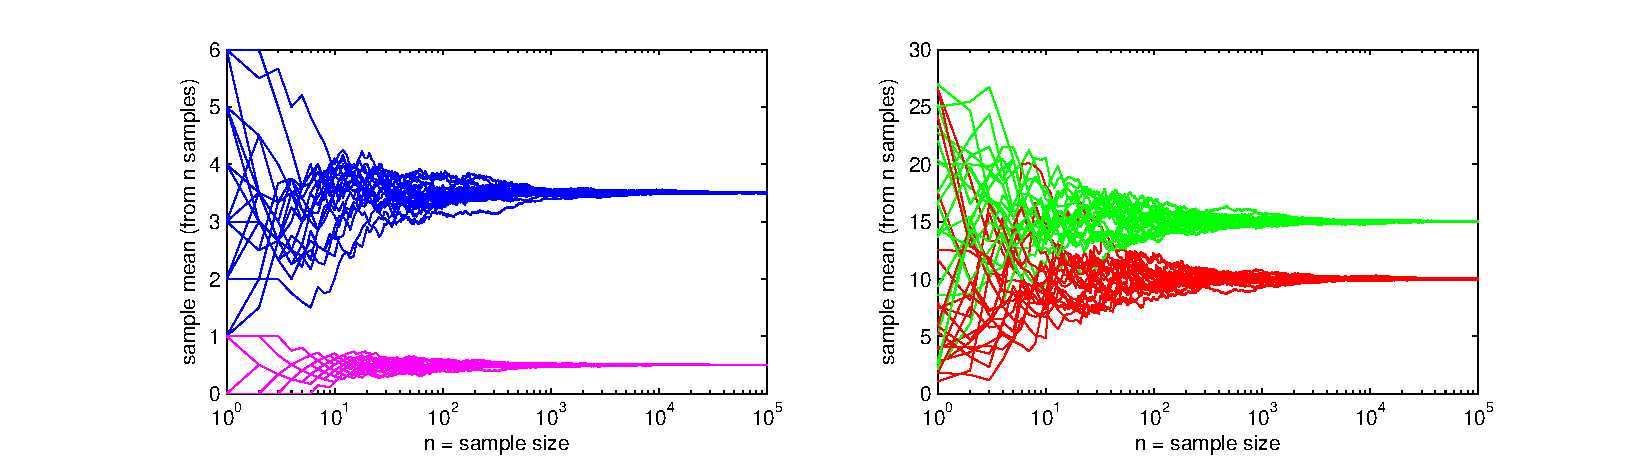
\includegraphics[width=6.5in]{figures/RunningMeansFairDieFairCoinUnif01Exp1By10}}
\end{figure}

\begin{example}[Bernoulli WLLN and Galton's Quincunx]\label{EgBernoulliWLLN}
We can appreciate the WLLN for $\overline{X}_n = n^{-1} S_n = \sum_{i=1}^{n} X_i$, where $X_1,X_2,\ldots,X_n \overset{\IID}{\sim} Bernoulli(p)$ using the paths of balls dropped into Galton's Quincunx of Sec.~\ref{S:Quincunx}.
\end{example}

\subsubsection{$\cauchy$ whose expectations does not exist has no Law of Large Numbers}

 Recall that the mean of the $\cauchy$ RV $X$ does not exist since $\int \left|x\right|\,dF(x) = \infty$ \eqref{E:CauchyMeanDoesNotExist}.  We will investigate this in \hyperref[LW:RunningMeanCauchy]{Labwork~\ref*{LW:RunningMeanCauchy}}.

 \begin{labwork}[Running mean of the Standard Cauchy RV]\label{LW:RunningMeanCauchy}
Let us see what happens when we plot the running sample mean for an increasing sequence of IID samples from the Standard Cauchy RV $X$ by implementing the following script file:
 \VrbMf[label=PlotStandardCauchyRunningMean.m]{scripts/PlotStandardCauchyRunningMean.m}

%}%end remove

\begin{figure}[htpb]
\caption{Unending fluctuations of  the running means based on $n$ IID samples from the Standard $\cauchy$ RV $X$ in each of five replicate simulations (blue lines).  The running means, based on $n$ IID samples from the $\uniform(0,10)$ RV, for each of five replicate simulations (magenta lines). \label{F:plot5RunningMeansStandardcauchyUnif010}}
\centering   \makebox{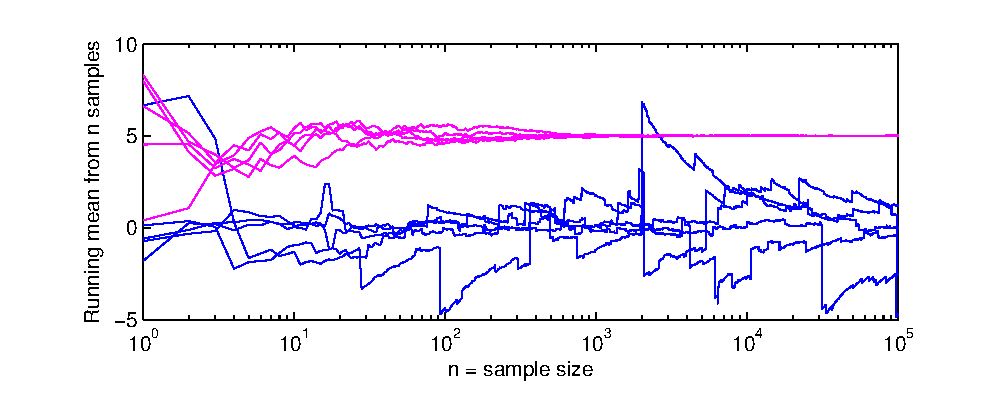
\includegraphics[width=5.5in]{figures/plot5RunningMeansStandardcauchyUnif010}}
\end{figure}

The resulting plot is shown in \hyperref[F:plot5RunningMeansStandardcauchyUnif010]{Figure~\ref*{F:plot5RunningMeansStandardcauchyUnif010}}.  Notice that the running means or the sample mean of $n$ samples as  a function of $n$, for each of the five replicate simulations, never settles down to a particular value.  This is because of the ``thick tails'' of the density function for this RV which produces extreme observations.  Compare them with the running means, based on $n$ IID samples from the $\uniform(0,10)$ RV, for each of five replicate simulations (magenta lines).  The latter sample means have settled down stably to the mean value of $5$ after about $700$ samples.
%\remove{
\end{labwork}
%}%end remove


\subsection{Application: Point Estimation of $E(X_1)$}
LLN gives us a method to obtain a {\bf point estimator} that gives ``the single best guess'' for the possibly unknown population mean $E(X_1)$ based on $\ol{X}_n$, the sample mean, of a simple random sequence (SRS) or independent and identically distributed (IID) sequence of $n$ RVs $X_1,X_2,\ldots, X_n \overset{IID}{\sim} X_1$.

\begin{example}\label{Eg:LLNExponential}
Let $X_1,X_2,\ldots, X_n \overset{IID}{\sim} X_1$, where $X_1$ is an $\exponential(\lambda^*)$ RV, i.e., let
\[
X_1,X_2,\ldots, X_n \overset{IID}{\sim} \exponential(\lambda^*) \enspace .
\]
Typically, we do not know the ``true'' parameter $\lambda^* \in \BB{\Lambda} = (0,\infty)$ or the population mean $E(X_1) = 1/\lambda^*$.  
But by LLN, we know that
\[
\ol{X}_n \rightsquigarrow \pointmass(E(X_1)) \enspace ,
\]
and therefore, we can use the sample mean $\ol{X}_n$ as a point estimator of $E(X_1)= 1/\lambda^*$.  

Now, suppose you model seven waiting times in nearest minutes between Orbiter buses at Balgay street as follows:
\[
X_1,X_2,\ldots, X_7 \overset{IID}{\sim} \exponential(\lambda^*) \enspace ,
\]
and have the following realization as your observed data:
\[
(x_1,x_2,\ldots,x_7) = (2,12,8,9,14,15,11) \enspace .
\]
Then you can use the observed sample mean $\ol{x}_7=(2+12+8+9+14+15+11)/7=71/7 \approxeq 10.14$ as a {\bf point estimate} of the population mean $E(X_1)=1/\lambda^*$.  
By the rearrangement $\lambda^*=1/E(X_1)$, we can also obtain a point estimate of the ``true'' parameter $\lambda^*$ from $1/\ol{x}_7=7/71 \approxeq 0.0986$. 
\end{example}

\begin{rem}[Point estimates are realizations of the Point Estimator]
We say the statistic $\ol{X}_n$, which is a random variable that depends on the data \rv~$(X_1,X_2,\ldots,X_n)$, is a {\bf point estimator} of $E(X_1)$.  
But once we have a realization of the data \rv~, i.e., our observed data vector $(x_1,x_2,\ldots,x_n)$ and its corresponding realization as observed sample mean $\ol{x}_n$, we say $\ol{x}_n$ is a {\bf point estimate} of $E(X_1)$.  In other words, the point estimate $\ol{x}_n$ is a realization of the the random variable $\ol{X}_n$ called the point estimator of $E(X_1)$.  
Therefore, when we observe a new data vector $(x'_1,x'_2,\ldots,x'_n)$  that is different from our first data vector $(x_1,x_2,\ldots,x_n)$, our point estimator of $E(X_1)$ is still $\ol{X}_n$ but the point estimate $n^{-1}\sum_{i=1}^nx'_i$ may be different from the first point estimate $n^{-1}\sum_{i=1}^nx_i$.  The sample means from $n$ samples for 20 replications (repeats of the experiment) are typically distinct especially for small $n$ as shown in Figure~\ref{F:RunningMeansFairDieFairCoinUnif01Exp1By10}.
\end{rem}

\begin{example}\label{Eg:LLNBernoulli}
Let $X_1,X_2,\ldots, X_n \overset{IID}{\sim} X_1$, where $X_1$ is an $\bernoulli(\theta^*)$ RV, i.e., let
\[
X_1,X_2,\ldots, X_n \overset{IID}{\sim} \bernoulli(\theta^*) \enspace .
\]
Typically, we do not know the ``true'' parameter $\theta^* \in \BB{\Theta} = [0,1]$, which is the same as the population mean $E(X_1) = \theta^*$.  
But by LLN, we know that
\[
\ol{X}_n \rightsquigarrow \pointmass(E(X_1)) \enspace ,
\]
and therefore, we can use the sample mean $\ol{X}_n$ as a point estimator of $E(X_1)= \theta^*$.  

Now, suppose you model seven coin tosses (encoding {\sf Heads} as $1$ with probability $\theta^*$ and {\sf Tails} as $0$ with probability $1-\theta^*$) as follows:
\[
X_1,X_2,\ldots, X_7 \overset{IID}{\sim} \bernoulli(\theta^*) \enspace ,
\]
and have the following realization as your observed data:
\[
(x_1,x_2,\ldots,x_7) = (0,1,1,0,0,1,0) \enspace .
\]
Then you can use the observed sample mean $\ol{x}_7=(0+1+1+0+0+1+0)/7=3/7 \approxeq 0.4286$ as a {\bf point estimate} of the population mean $E(X_1)=\theta^*$.  
Thus, our ``single best guess'' for $E(X_1)$ which is the same as the probability of {\sf Heads} is $\ol{x}_7=3/7$.  
\end{example}

Of course, if we tossed the same coin in the same IID manner another seven times or if we observed another seven waiting times of orbiter buses at a different bus-stop or on a different day we may get a different point estimate for $E(X_1)$.  
See the intersection of the twenty magenta sample mean trajectories for simulated tosses of a fair coin from IID $\bernoulli(\theta^*=1/2)$ RVs and the twenty red sample mean trajectories for simulated waiting times from IID $\exponential(\lambda^*=1/10)$ RVs in Figure~\ref{F:RunningMeansFairDieFairCoinUnif01Exp1By10} with $n=7$.  
Clearly, the point estimates for such a small sample size are fluctuating wildly!  
However, the fluctuations in the point estimates settles down for larger sample sizes.  


The {\em next natural question is how large should the sample size be} in order to have a small interval of width, say $2 \epsilon$, ``contain'' $E(X_1)$, the quantity of interest, with a high probability, say $1-\alpha$?  If we can answer this then we can make probability statements like the following:
\[
P( \mathsf{error} < \mathsf{tolerance}) = P( |\ol{X}_n - E(X_1)| < \epsilon ) = P(-\epsilon < \ol{X}_n - E(X_1) < \epsilon) = 1-\alpha \enspace .
\]

In order to ensure the $\mathsf{error}=|\ol{X}_n - E(X_1)|$ in our estimate of $E(X_1)$ is within a required $\mathsf{tolerance}=\epsilon$ we need to know the full distribution of $\ol{X}_n - E(X_1)$ itself.  The Central Limit Theorem (CLT) helps us here.


\section{Central Limit Theorem}

What if we scale the sum of $X_i$`s by $\sqrt{n}$ instead of $n$?

\begin{Exercise}[title={What if we scale by $\sqrt{n}$},label={xSumOFUnifminu1To1DividedBySqrtn}]
After reading Sec.~\ref{S:ConvOfRVs} up to now, think carefully about what you need to be able to show that $Z_n := 1/\sqrt{n}\sum_{i=1}^n X_i$ converges in distribution to the $\normal(0,1/3)$ RV, where $X_i \overset{IID}{\sim} \uniform(-1,1)$. {Hint: Characteristic functions}
%\ExePart
%\Question
%\subQuestion Show that...
%\subQuestion In this question...
%\subsubQuestion Show that...
%\subsubQuestion Conclude...
%\subQuestion Conclude.
%\Question Show that if $b > 1$...
%\ExePart
%\Question What happens to if $b=1$?
\end{Exercise}

\remove{ % removing CSE book CLT without proof
\begin{prop}[Central Limit Theorem (CLT)]
Let $X_1,X_2,\ldots \overset{\IID}{\sim} X_1$ and suppose $\e(X_1)$ and $\V(X_1)$ exists, then 
{\small
\begin{eqnarray}
%1
\overline{X}_n = \frac{1}{n} \sum_{i=1}^n X_i 
& \rightsquigarrow & 
X \sim \normal \left( \e(X_1),\frac{\V(X_1)}{n}  \right) \ , \\
%2
\overline{X}_n -\e(X_1) 
& \rightsquigarrow & 
X-\e(X_1) \sim \normal \left( 0,\frac{\V(X_1)}{n}  \right) \ , \\
%3
\sqrt{n} \left( \overline{X}_n -\e(X_1) \right)
& \rightsquigarrow & 
\sqrt{n} \left( X-\e(X_1) \right) \sim \normal \left( 0,\V(X_1)  \right) \ , \\
%4
Z_n :=  \frac{\overline{X}_n-\e(\overline{X}_n)}{\sqrt{\V(\overline{X}_n)}} 
= \frac{\sqrt{n} \left( \overline{X}_n -\e(X_1) \right)}{\sqrt{\V(X_1)}}
& \rightsquigarrow & 
Z  \sim \normal \left( 0,1  \right) \ , \\
%5
\lim_{n \to \infty} P\left( \frac{\overline{X}_n-\e(\overline{X}_n)}{\sqrt{\V(\overline{X}_n)}}  \leq z \right)
= \lim_{n \to \infty} \p(Z_n \leq z)
&=&
\Phi(z) := \int_{- \infty}^z \left( \frac{1}{\sqrt{2 \pi}} \ \exp \left( \frac{-x^2}{2} \right) \right) dx \ .
\end{eqnarray}
}
Thus, for sufficiently large $n$ (say $n>30$) we can make the following approximation:
\begin{equation}\label{E:CLTApprox}
P\left( \frac{\overline{X}_n-\e(\overline{X}_n)}{\sqrt{\V(\overline{X}_n)}}  \leq z \right) 
\approxeq 
\p(Z \leq z)
=
\Phi(z) := \int_{- \infty}^z \left( \frac{1}{\sqrt{2 \pi}} \ \exp \left( \frac{-x^2}{2} \right) \right) dx \ .
\end{equation}
{\scriptsize
\begin{proof}
See any intermediate to advanced undergraduate text in Probability.  Start from the index looking for ``Central Limit Theorem'' to find the page number for the proof \ldots .
\end{proof}
}
{\bf Heuristic Interpretation of CLT:}  Probability statements about the sample mean RV $\overline{X}_n$ can be approximated using a Normal distribution. 
\end{prop}
Here is a simulation showing CLT in action.
\begin{VrbM}
>> % a demonstration of Central Limit Theorem --
>> % the sample mean of a sequence of n IID Exponential(lambda) RVs 
>> % itself a Gaussian(1/lambda,lambda/n) RV
>> lambda=0.1; Reps=10000; n=10; hist(sum(-1/lambda * log(rand(n,Reps)))/n)
>> lambda=0.1; Reps=10000; n=100; hist(sum(-1/lambda * log(rand(n,Reps)))/n,20)
>> lambda=0.1; Reps=10000; n=1000; hist(sum(-1/lambda * log(rand(n,Reps)))/n,20)
\end{VrbM}

Let us look at an example that makes use of the CLT next.
\begin{example}[Errors in computer code (Wasserman03, p.~78)]\label{EX:CLTPoisson}
Suppose the collection of RVs $X_1,X_2, \ldots, X_n$ model the number of errors in $n$ computer programs named $1,2,\ldots,n$, respectively.  Suppose that the RV $X_i$ modeling the number of errors in the $i$-th program is the $Poisson(\lambda=5)$ for any $i=1,2,\ldots,n$.  Further suppose that they are independently distributed.  Succinctly, we suppose that 
\[
X_1,X_2,\ldots,X_n \overset{\IID}{\sim} \poisson(\lambda=5) \ . 
\]
Suppose we have $n=125$ programs and want to make a probability statement about $\overline{X}_n$ which is the average error per program out of these $125$ programs.  Since $\e(X_i) = \lambda=5$ and $\V(X_i)=\lambda=5$, we may want to know how often our sample mean $\overline{X}_{125}$ differs from the expectation of $5$ errors per program.  Using the CLT we can approximate $\p(\overline{X}_n < 5.5)$, for instance, as follows:
\begin{eqnarray}
\p(\overline{X}_n < 5.5) 
&=& P \left( \frac{\sqrt{n}(\overline{X}_n - \e(X_1))}{\sqrt{\V(X_1)}} < \frac{\sqrt{n}(5.5-\e(X_1))}{\sqrt{\V(X_1)}} \right) \notag \\
&\approxeq& P \left( Z < \frac{\sqrt{n}(5.5-\lambda)}{\sqrt{\lambda}} \right) \qquad \text{{\scriptsize [by \eqref{E:CLTApprox}, and $\e(X_1)=\V(X_1)=\lambda$]}} \notag \\
&=& P \left( Z < \frac{\sqrt{125}(5.5-5)}{\sqrt{5}} \right) \qquad \text{{\scriptsize [Since, $\lambda=5$ and $n=125$ in this Example]}} \notag \\
&=& \p(Z \leq 2.5) = \Phi(2.5) =  \int_{- \infty}^{2.5} \left( \frac{1}{\sqrt{2 \pi}} \ \exp \left( \frac{-x^2}{2} \right) \right) dx \approxeq 0.993790334674224 \ . \notag
\end{eqnarray}
The last number above needed the following:
\begin{labwork}[Numerical approximation of $\Phi(2.5)$]
The numerical approximation of $\Phi(2.5)$ was obtained via the following call to our $\erf$-based {\tt NormalCdf} function. % from \ref*{Mf: NormalCdfPdf}. MATLABback
\begin{VrbM}
>> format long
>> disp(NormalCdf(2.5,0,1))
   0.993790334674224
\end{VrbM}
\end{labwork}
\end{example}
The CLT says that if $X_1,X_2,\ldots \overset{\IID}{\sim} X_1$, then $Z_n := \sqrt{n}(\overline{X}_n-\e(X_1))/\sqrt{\V(X_1)}$ is approximately distributed as $\normal(0,1)$.  In \hyperref[EX:CLTPoisson]{Example \ref*{EX:CLTPoisson}}, we knew $\sqrt{\V(X_1)}$.   However, in general, we may not know $\sqrt{\V(X_1)}$.  The next proposition says that we may estimate $\sqrt{\V(X_1)}$ using the sample standard deviation $S_n$ of $X_1,X_2,\ldots,X_n$, according to \eqref{E:SampleStdDevRV}, and still make probability statements about the sample mean $\overline{X}_n$ using a Normal distribution.
\begin{prop}[CLT based on Sample Variance]
Let $X_1,X_2,\ldots \overset{\IID}{\sim} X_1$ and suppose $\e(X_1)$ and $\V(X_1)$ exists, then
\begin{equation}\label{E:CLTApproxSn}
\frac{\sqrt{n} \left( \overline{X}_n - \e(X_1) \right)}{S_n} \rightsquigarrow \normal(0,1) \ .
\end{equation}
\end{prop}

We will use \eqref{E:CLTApproxSn} for statistical estimation in the sequel.
}% end remove

%The next proposition is often referred to as the fundamental theorem of statistics and is at the heart of non-parametric inference, empirical processes, and computationally-intensive bootstrap techniques.
%\begin{prop}[Gilvenko-Cantelli Theorem]\label{P:Gilvenko-Cantelli}
%Let $X_1,X_2,\ldots,X_n \overset{\IID}{\sim} F$.  Then,
%\[
%\sup_x { | \widehat{F}_n(x) - F(x) | } \overset{\p}{\longrightarrow} 0 \ .
%\]
%{\scriptsize
%\begin{proof}
%Proof to be seen in STAT 318 or another advanced Statistics course.
%\end{proof}
%}
%\end{prop}
%{\bf Heuristic Interpretation of Gilvenko-Cantelli Theorem}:  As the sample size $n$ increases the empirical distribution function $\widehat{F}_n$ converges to the true DF $F$ in probability.

%\begin{figure}[htpb]
%\caption{Plots of ten distinct ECDFs $\widehat{F}_n$ based on $10$ sets of $n$ IID samples from $\uniform(0,1)$ RV $X$, as $n$ increases from $10$ to $100$ to $1000$.  The DF $F(x)=x$ over $[0,1]$ is shown in red.  The script of \hyperref[Mf:GilvenkoCantelliUnif01n10n100n100ECDFs]{Labwork \ref*{Mf:GilvenkoCantelliUnif01n10n100n100ECDFs}} was used to generate this plot.   \label{F:GilvenkoCantelliUnif01n10n100n100ECDFs}}
%\centering   \makebox{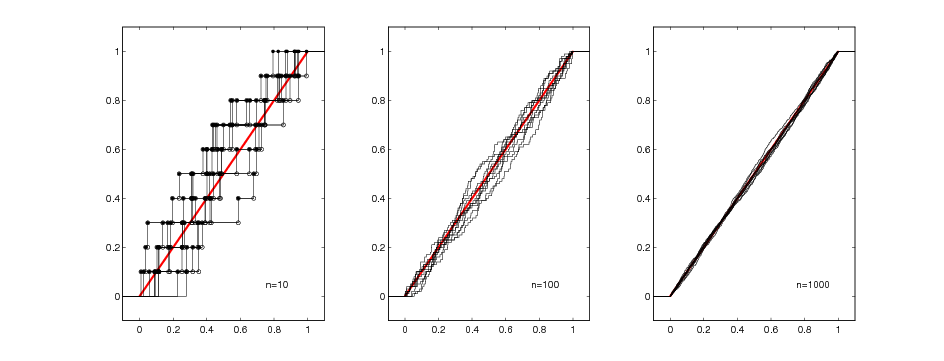
\includegraphics[width=7.0in]{figures/GilvenkoCantelliUnif01n10n100n100ECDFs}}
%\end{figure}

%\begin{prop}[The Dvoretzky-Kiefer-Wolfowitz (DKW) Inequality]
%Let $X_1,X_2,\ldots,X_n \overset{\IID}{\sim} F$.  Then, for any $\epsilon>0$,
%\begin{equation}\label{E:DKWNeq}
%P \left( \sup_x | \widehat{F}_n(x) - F(x) | > \epsilon  \right) \leq 2 \exp {(-2 n \epsilon^2)}
%\end{equation}
%\end{prop}



\begin{prop}[Central Limit Theorem (CLT)]\label{P:CLT}

If we are given a sequence of independently and identically distributed (IID) RVs, $X_1,X_2,\ldots \overset{\IID}{\sim} X_1$ and if $E(X) < \infty$ and $V(X_1)<\infty$, then the sample mean $\overline{X}_n$ converges in 
%probability 
distribution to the Normal RV with mean given by any one of the IID RVs, say $\e(X_1)$ by convention, and variance given by $\frac{1}{n}$ times the variance of any one of the IID RVs, say $V(X_1)$ by convention.  More formally, we write:
\begin{multline}\label{E:CLT}
\text{If} \quad X_1,X_2,\ldots \overset{\IID}{\sim} X_1 \ \text{and if } \ \e(X_1)<\infty, V(X_1) < \infty \\ \text{ then } \ \overline{X}_n \rightsquigarrow \normal\left(E(X_1), \frac{V(X_1)}{n}\right) \ \text{ as } n\to\infty \enspace ,
\end{multline}
or equivalently after standardization:
\begin{multline}\label{E:CLTStd}
\text{If} \quad X_1,X_2,\ldots \overset{\IID}{\sim} X_1 \ \text{and if } \ \e(X_1)<\infty, V(X_1) < \infty \\ \text{ then } \ \frac{\overline{X}_n - E(X_1)}{\sqrt{V(X_1)/n}} \rightsquigarrow Z \sim \normal\left(0,1 \right) \ \text{ as } n\to\infty \enspace .
\end{multline}

{\normalsize
\begin{proof}
{
Our proof is based on the convergence of characteristic functions (CFs).  
We will prove the standardized form of the CLT in Equation~\eqref{E:CLTStd} by showing that the CF of
\[
U_n := \frac{\ol{X}_n-E(X_1)}{\sqrt{V(X_1)/n}}
\]
converges to the CF of $Z$, the $\normal(0,1)$ RV.  
First, note from Equation~\eqref{E:cfStandardNormal} that the CF of $Z \sim \normal(0,1)$ is:
\[
\cf_Z(t) = E \left( e^{\imath t Z}\right) = e^{-t^2/2} \enspace .
\]
Second, 
\[
U_n := \frac{\ol{X}_n-E(X_1)}{\sqrt{V(X_1)/n}} 
= \frac{\sum_{k=1}^n X_k - n E(X_1)}{\sqrt{nV(X_1)}}
= \frac{1}{\sqrt{n}} \sum_{k=1}^n \left(\frac{X_k - E(X_1)}{\sqrt{V(X_1)}}\right)\enspace .
\]
Therefore, the CF of $U_n$ is
\begin{align*}
\cf_{U_n}(t) 
&= E\left( \exp\left({\imath t U_n}\right)\right)
= E \left( \exp\left({\imath \frac{t}{\sqrt{n}}\sum_{k=1}^n \frac{X_k - E(X_1)}{\sqrt{V(X_1)}} }\right)\right)
= \prod_{k=1}^n E \left( \exp \left( \imath \frac{t}{\sqrt{n}} \frac{X_k - E(X_1)}{\sqrt{V(X_1)}} \right) \right)\\
&= \left( E \left( \exp \left( \imath \frac{t}{\sqrt{n}} \frac{X_1 - E(X_1)}{\sqrt{V(X_1)}} \right) \right)\right)^n \enspace .
\end{align*}
Now, if we let
\[
Y = \frac{X_1 - E(X_1)}{\sqrt{V(X_1)}}
\]
then 
\[
E(Y) = 0 \, , \quad E(Y^2)=1 \, , \text{and} \quad V(Y)=1 \enspace . 
\]
So, the CF of $U_n$ is
\[
\cf_{U_n}(t) = \left( \cf_Y\left(\frac{t}{\sqrt{n}}\right)\right)^n \enspace ,
\]
and since we can Taylor expand $\cf_Y(t)$ as follows: 
\[
\cf_Y(t) = 1 + \imath t E(Y) + \imath^2 \frac{t^2}{2} E(Y^2) + o(t^2) \enspace,
\]
which implies
\[
\cf_Y\left(\frac{t}{\sqrt{n}}\right) = 1 + \frac{\imath t}{\sqrt{n}} E(Y) + \frac{\imath^2 t^2}{2n}  E(Y^2) + o\left(\frac{t^2}{n}\right) \enspace,
\]
we finally get
\[
\cf_{U_n}(t) 
= \left( \cf_Y \left(\frac{t}{\sqrt{n}}\right) \right)^n
= \left( 1 +  \frac{\imath t}{\sqrt{n}} \times 0 + \frac{\imath^2 t^2}{2n}  \times 1 + o\left(\frac{t^2}{n}\right) \right)^n
= \left( 1 - \frac{t^2}{2n} + o\left(\frac{t^2}{n}\right) \right)^n
\to e^{-t^2/2} = \cf_Z(t) \enspace .
\]
For the last limit we have used $\left( 1+\frac{x}{n}\right)^n \to e^x$ as $n \to \infty$.  
Thus, we have proved Equation~\eqref{E:CLTStd} which is equivalent to Equation~\eqref{E:CLT} by a standardization argument that if $W \sim \normal(\mu,\sigma^2)$ then $Z=\frac{W-\mu}{\sigma} \sim \normal(0,1)$ through the linear transformation $W=\sigma Z + \mu$ of Example~\ref{Eg:LinearTransfStdGaussianGaussian}.
}
\end{proof}
}
\end{prop}


\subsection{Application: Tolerating Errors in our estimate of $E(X_1)$}
Recall that we wanted to ensure the $\mathsf{error}=|\ol{X}_n - E(X_1)|$ in our estimate of $E(X_1)$ is within a required $\mathsf{tolerance}=\epsilon$ and make the following probability statement: 
\[
P( \mathsf{error} < \mathsf{tolerance}) = P( |\ol{X}_n - E(X_1)| < \epsilon ) = P(-\epsilon < \ol{X}_n - E(X_1) < \epsilon) = 1-\alpha \enspace .
\]
To be able to do this we needed to know the full distribution of $\ol{X}_n - E(X_1)$ itself.  

Due to the Central Limit Theorem (CLT) we now know that (assuming $n$ is large)
\begin{align*}
P(-\epsilon < \ol{X}_n - E(X_1) < \epsilon) 
&\approxeq P\left(-\frac{\epsilon}{\sqrt{V(X_1)/n}} < \frac{\ol{X}_n - E(X_1)}{\sqrt{V(X_1)/n}} < \frac{\epsilon}{\sqrt{V(X_1)/n}}\right)\\
&= P\left(-\frac{\epsilon}{\sqrt{V(X_1)/n}} < Z < \frac{\epsilon}{\sqrt{V(X_1)/n}} \right) \enspace ,
\end{align*}
where $Z \sim \normal(0,1)$.

\begin{example}\label{EgProbOfErrorInMeanEstimateFromKnownVar}
Suppose an IID sequence of observations $(x_1,x_2,\ldots,x_{80})$ was drawn from a distribution with variance $V(X_1)=4$.  
What is the probability that the error in $\ol{x}_n$ used to estimate $E(X_1)$ is less than $0.1$?

By CLT,
\[
P (\mathsf{error} < 0.1) \approxeq P \left( -\frac{0.1}{\sqrt{4/80}} < Z < \frac{0.1}{\sqrt{4/80}} \right) 
= P(-0.447 < Z < 0.447)= 0.345 \enspace .
\] 
\end{example}

Suppose you want the $\mathsf{error}$ to be less than $\mathsf{tolerance}=\epsilon$ with a certain probability $1-\alpha$.  
Then we can use CLT to do such {\bf sample size calculations}.
Recall the DF $\Phi(z) = P(Z < z)$ is tabulated in the standard normal table and now we want
\[
P \left(-\frac{\epsilon}{\sqrt{V(X_1)/n}} < Z < \frac{\epsilon}{\sqrt{V(X_1)/n}} \right) = 1 -\alpha \enspace .
\]
We know,
\[
P \left(-z_{\alpha/2} < Z < z_{\alpha/2} \right) = 1 -\alpha \enspace ,
\]

\vspace{1.5cm}

{\tiny make the picture here of $f_Z(z) = \Phi'(z)$ to recall what $z_{\alpha/2}$, $z_{-\alpha/2}$, and the various areas below $f_Z(\cdot)$ in terms of $\Phi(\cdot)$ from the table really mean... (See Example~\ref{Eg:UsingNormalTables}).}

\vspace{1.5cm}

where, $\Phi(z_{\alpha/2}) = 1-\alpha/2$ and $\Phi(z_{-\alpha/2}) = 1- \Phi(z_{\alpha/2}) = \alpha/2$.  
So, we set
\[
\frac{\epsilon}{\sqrt{V(X_1)/n}} = z_{\alpha/2}
\]
and rearrange to get
\begin{equation}\label{E:SampleSizeCalcForPopMean}
n = \left( \frac{\sqrt{V(X_1)} z_{\alpha/2}}{\epsilon}\right)^2
\end{equation}
for the needed sample size that will ensure that our $\mathsf{error}$ is less than our $\mathsf{tolerance}=\epsilon$ with probability $1-\alpha$.  Of course, if $n$ given by Equation~\eqref{E:SampleSizeCalcForPopMean} is not a natural number then we naturally round up to make it one!

A useful $z_{\alpha/2}$ value to remember: If $\alpha=0.05$ when the probability of interest $1-\alpha=0.95$ then $z_{\alpha/2} = z_{0.025} = 1.96$.

\begin{example}\label{EgHowLargeASampleSizeToEstimateMeanWithinTOL}
How large a sample size is needed to make the $\mathsf{error}$ in our estimate of the population mean $E(X_1)$ to be less than $0.1$ with probability $1-\alpha=0.95$ if we are observing IID samples from a distribution with a population variance $V(X_1)$ of $4$?

Using Equation~\eqref{E:SampleSizeCalcForPopMean} we see that the needed sample size is
\[
n =  \left( \frac{\sqrt{4} \times 1.96}{0.1} \right)^2 \approxeq 1537
\]
Thus, it pays to check the sample size needed in advance of experimentation, provided you already know the population variance of the distribution whose population mean you are interested in estimating within a given $\mathsf{tolerance}$ and with a high probability. 
\end{example}

\subsection{Application: Set Estimation of $E(X_1)$}

A useful byproduct of the CLT is the $\mathbf{(1-\alpha)}$ {\bf confidence interval}, a random interval (or bivariate \rv) that contains $E(X_1)$, the quantity of interest, with probability $1-\alpha$: 
\begin{equation}\label{E:ConfIntForPopMean}
\left( \ol{X}_n \pm z_{\alpha/2} \sqrt{V(X_1)/n} \right) :=
\left( \ol{X}_n - z_{\alpha/2} \sqrt{V(X_1)/n} \, , \, \ol{X}_n + z_{\alpha/2} \sqrt{V(X_1)/n} \right) \enspace .
\end{equation}

{\scriptsize
We can easily see how Equation~\eqref{E:ConfIntForPopMean} is derived from CLT as follows:
\begin{align*}
P \left( -z_{\alpha/2} < Z < z_{\alpha/2} \right) 
&= 1-\alpha \\
P \left( -z_{\alpha/2} < \frac{\ol{X}_n-E(X_1)}{\sqrt{V(X_1)/n}} < z_{\alpha/2} \right) 
&= 1-\alpha \\
P \left( -\ol{X}_n - z_{\alpha/2}\sqrt{V(X_1)/n}  < -E(X_1) < -\ol{X}_n + z_{\alpha/2} \sqrt{V(X_1)/n} \right) 
&= 1-\alpha \\
P \left( \ol{X}_n + z_{\alpha/2}\sqrt{V(X_1)/n}  > E(X_1) > \ol{X}_n - z_{\alpha/2} \sqrt{V(X_1)/n} \right) 
&= 1-\alpha \\
P \left( \ol{X}_n - z_{\alpha/2}\sqrt{V(X_1)/n}  < E(X_1) < \ol{X}_n + z_{\alpha/2} \sqrt{V(X_1)/n} \right) 
&= 1-\alpha \\
P \left( E(X_1) \in \left(\ol{X}_n - z_{\alpha/2}\sqrt{V(X_1)/n} , \ol{X}_n + z_{\alpha/2} \sqrt{V(X_1)/n} \right) \right) 
&= 1-\alpha \enspace .
\end{align*}
}

\begin{rem}[Heuristic interpretation of the $(1-\alpha)$ confidence interval]  
If we repeatedly produced samples of size $n$ to contain $E(X_1)$ within a $\left( \ol{X}_n \pm z_{\alpha/2} \sqrt{V(X_1)/n} \right)$, say $100$ times, then on average, $(1-\alpha) \times 100$ repetitions will actually contain $E(X_1)$ within the random interval and $\alpha \times 100$ repetitions will fail to contain $E(X_1)$.
\end{rem}

So far, we have assumed we know the population variance $V(X_1)$ in an IID experiment with $n$ samples and tried to estimate the population mean $E(X_1)$.  
But in general, we will not know $V(X_1)$.  We can still get a point estimate of $E(X_1)$ from the sample mean due to LLN but we won't be able to get a confidence interval for $E(X_1)$.  
Fortunately, a more elaborate form of the CLT tells us that even when we substitute the sample variance $S_n^2 = \frac{1}{n-1}\sum_{i=1}^n (X_i-\ol{X}_n)^2$ for the population variance $V(X_1)$ the following $1-\alpha$ confidence interval for $E(X_1)$ works!
\begin{equation}\label{E:ConfIntForPopMeanUsingSampleVariance}
\left( \ol{X}_n \pm z_{\alpha/2} S_n/\sqrt{n} \right) :=
\left( \ol{X}_n - z_{\alpha/2} S_n/\sqrt{n} \, , \, \ol{X}_n + z_{\alpha/2} S_n/\sqrt{n} \right) \enspace ,
\end{equation}
where, $S_n=\sqrt{S_n^2}$ is the sample standard deviation.

Let's return to our two examples again.

\begin{example}\label{EgExponentialCIOfMeanWaitingTimesWithSampleMeanAndVar}
We model the waiting times between Orbiter buses with unknown $E(X_1)=1/\lambda^*$ as
\[
X_1,X_2,\ldots,X_n \overset{IID}{\sim} \exponential(\lambda^*)
\]
and observed the following data, sample mean, sample variance and sample standard deviation:
\[
(x_1,x_2,\ldots,x_7) = (2,12,8,9,14,15,11), \, \ol{x}_7=10.143, \,  s^2_7 = 19.143, \, s_7 = 4.375 \enspace ,
\] 
respectively.  
Our point estimate and $1-\alpha=95\%$ confidence interval for $E(X_1)$ are:
\[
\ol{x}_7 = 10.143 \quad \text{ and } \quad (\ol{x}_7 \pm z_{\alpha/2} s_7/\sqrt{7}) = (10.143 \pm 1.96 \times 4.375/\sqrt{7}) = (6.9016,13.3841) \enspace ,
\]
respectively.  So with $95\%$ probability the true population mean $E(X_1)=1/\lambda^*$ is contained in $(6.9016,13.3841)$ and since the mean waiting time of $10$ minutes promised by the Orbiter bus company is also within $(6.9016,13.3841)$ we can be fairly certain that the company sticks to its promise.
\end{example}

\begin{example}\label{EgBernoulliCIWithSampleMeanAndVar}
We model the tosses of a coin with unknown $E(X_1)=\theta^*$ as
\[
X_1,X_2,\ldots,X_n \overset{IID}{\sim} \bernoulli(\theta^*)
\]
and observed the following data, sample mean, sample variance and sample standard deviation:
\[
(x_1,x_2,\ldots,x_7) = (0,1,1,0,0,1,0), \, \ol{x}_7=0.4286, \,  s^2_7 = 0.2857, \, s_7 = 0.5345 \enspace ,
\] 
respectively.  
Our point estimate and $1-\alpha=95\%$ confidence interval for $E(X_1)$ are:
\[
\ol{x}_7 = 0.4286 \quad \text{ and } \quad (\ol{x}_7 \pm z_{\alpha/2} s_7/\sqrt{7}) = (0.4286 \pm 1.96 \times 0.5345/\sqrt{7}) = (0.0326,0.8246) \enspace ,
\]
respectively.  So with $95\%$ probability the true population mean $E(X_1)=\theta^*$ is contained in $(0.0326,0.8246)$ and since $1/2$ is contained in this interval of width $0.792$ we cannot rule out that the flipped coin is not fair with $\theta^*=1/2$.
\end{example}

\begin{rem}
The normal-based confidence interval for $\theta^*$ (as well as $\lambda^*$ in the previous example) may not be a valid approximation here with just $n=7$ samples.  After all, the CLT only tells us that the point estimator $\widehat{\Theta}_n$ can be approximated by a normal distribution for large sample sizes. 
When the sample size $n$ was increased from $7$ to $100$ by tossing the same coin another $93$ times, a total of $57$ trials landed as Heads.  Thus the point estimate and confidence interval for $E(X_1)=\theta^*$ based on the sample mean and sample standard deviations are:
\[
\widehat{\theta}_{100} = \frac{57}{100} = 0.57 \qquad \text{and} \qquad
 (0.57 \pm 1.96 \times 0.4975/\sqrt{100})
 =(0.4725, 0.6675) \enspace .
\]
Thus our confidence interval shrank considerably from a width of $0.792$ to $0.195$ after an additional $93$ Bernoulli trials.  Thus, we can make the width of the confidence interval as small as we want by making the number of observations or sample size $n$ as large as we can.
\end{rem}

%%%%%%%%%%%%%%%%%%%%%%%%%%%%%%%%%%%%%%%%%%%%%%%%%%%%%%%%%%%%%%%%%%%%%%%%%%%%%%%%%%%%%%%%%%%%%

\section{Exercises in Limit Laws of Statistics}\label{S:xsLimitLaws}% {S:xsCFs}% {S:xsExpectationsOfRVs} %S:xsMultivariateRVs

\begin{ExerciseList}

\Exercise
Suppose you plan to obtain a simple random sequence (SRS) --- also known as independent and identically distributed (IID) sequence --- of $n$ measurements from an instrument.  
This instrument has been calibrated so that the distribution of measurements made with it have population variance of $1/4$.  
Your boss wants you to make a point estimate of the unknown population mean from a SRS of sample size $n$.  
He also insists that the tolerance for error has to be $1/10$ and the probability of meeting this tolerance should be just above $95\%$.  
Use CLT to find how large should $n$ be to meet the specifications of your boss.
\Answer
~\\
%Using the CLT implied Equation (61) in the lecture notes and further noting from the Standard Normal Table that when $z_{\alpha/2}=2$ we get the desired $1-\alpha=0.9772>0.95$ we get
%\[
%n = \left( \sqrt{(V(X_1)} z_{\alpha/2}) / \epsilon \right)^2 = \left( (\sqrt{1/4}\times 2) / (1/10) \right)^2
%= \left( ((1/2)\times 2) / (1/10) \right)^2 = 10^2 = 100
%\]
We want $1-\alpha = 0.95$, and from the standard Normal Table we know that the corresponding $z_{\alpha/2}=1.96$.   
Then we can get the right sample size $n$ from the CLT implied Equation (61) in the lecture notes, which is,
\[
n = \left( \sqrt{(V(X_1)} z_{\alpha/2}) / \epsilon \right)^2 \enspace ,
\] 
as follows:
\begin{eqnarray*}
n &= \left( \sqrt{(V(X_1)} z_{\alpha/2}) / \epsilon \right)^2 = \left( (\sqrt{1/4}\times 1.96) / (1/10) \right)^2\\
&= \left( ((1/2)\times 1.96) / (1/10) \right)^2 = (0.98 \times 10)^2 = 9.8^2 = 96.04
\end{eqnarray*}
Finally, by rounding $96.04$ up to the next largest integer we need $n=97$ measurements to meet the specifications of your boss (at least up to the approximation provided by the CLT).


\Exercise 
Suppose the collection of RVs $X_1,X_2, \ldots, X_n$ model the number of errors in $n$ computer programs named $1,2,\ldots,n$, respectively.  Suppose that the RV $X_i$ modeling the number of errors in the $i$-th program is the $\textrm{Poisson}(\lambda=5)$ for any $i=1,2,\ldots,n$.  Further suppose that they are independently distributed.  Succinctly, we suppose that 
\[
X_1,X_2,\ldots,X_n \overset{\IID}{\sim} \poisson(\lambda=5) \ . 
\]
Suppose we have $n=125$ programs and want to make a probability statement about $\overline{X}_{125}$ which is the average error per program out of these $125$ programs.  Since $E(X_i) = \lambda=5$ and $V(X_i)=\lambda=5$, we want to know how often our sample mean $\overline{X}_{125}$ differs from the expectation of $5$ errors per program.  
Using the CLT find the $P(\overline{X}_{125} < 5.5)$.
\Answer
~\\
By CLT, $\frac{\sqrt{n}(\overline{X}_n - \E(X_1))}{\sqrt{\V(X_1)}} \rightsquigarrow Z \sim \mathrm{Normal}(0,1)$.  
So we need to apply the ``standardization'' to both sides of the inequality that is defining the event of interest:
$$\{\overline{X}_n < 5.5\} \enspace ,$$ 
in order to find its probability $\P(\overline{X}_n < 5.5)$.
~\\
\begin{eqnarray}
\P(\overline{X}_n < 5.5) 
&=& P \left( \frac{\sqrt{n}(\overline{X}_n - \E(X_1))}{\sqrt{\V(X_1)}} < \frac{\sqrt{n}(5.5-\E(X_1))}{\sqrt{\V(X_1)}} \right) \notag \\
&\approxeq& P \left( Z < \frac{\sqrt{n}(5.5-\lambda)}{\sqrt{\lambda}} \right) \qquad \text{{\scriptsize [
since we know/assume that $\E(X_1)=\V(X_1)=\lambda$]}} \notag \\
&=& P \left( Z < \frac{\sqrt{125}(5.5-5)}{\sqrt{5}} \right) \qquad \text{{\scriptsize [Since, $\lambda=5$ and $n=125$ in this Example]}} \notag \\
&=& \P(Z \leq 2.5) = \Phi(2.5) = 0.9938\ . \notag
\end{eqnarray}
(source: Wasserman, {\em All of Statistics}, Springer, p.~78, 2003)


\Exercise
What is the distribution of $\sum_{i=1}^n{X_i}/n$ as $n \to \infty$ when $X_i \overset{IID}{\sim} \uniform(-10,10)$?
\Answer
HINT: Use the LLN after finding the population mean of $X_i$.
\Exercise
What is the distribution of $\sum_{i=1}^n{X_i}/\sqrt{\V(X_i)n}$ as $n \to \infty$ when $X_i \overset{IID}{\sim} \uniform(-10,10)$?
\Answer
HINT: Use the CLT after finding the population mean and variance of $X_i$.
\end{ExerciseList}

